\documentclass[11pt]{article}
\usepackage[utf8]{inputenc}
\usepackage[T1]{fontenc}
\usepackage{amsmath}
\usepackage{amssymb}
\usepackage{multicol}
\usepackage{geometry}
\usepackage{tikz}
\usepackage{enumitem}
\usepackage{xcolor}
\usepackage{titlesec}
\usepackage{tcolorbox}
\tcbset{enhanced, boxrule=0.8pt, arc=4pt, auto outer arc}

% Configurações de layout
\geometry{a4paper, left=1cm, right=1cm, top=0.5cm, bottom=1.2cm}
\setlength{\columnseprule}{0.4pt}

% Cores para títulos
\titleformat{\section}{\normalfont\Large\bfseries\color{blue}}{\thesection}{1em}{}
\titleformat{\subsection}{\normalfont\large\bfseries\color{red}}{\thesubsection}{1em}{}

\title{\textcolor{orange}{Terceiro Trimestre: Matemática
    \\Progressão Geométrica - Revisão}}
\author{Professor: Jefferson}
\date{}

\begin{document}

\maketitle
\vspace{-1cm}

%\begin{center}
%\large{Nome: \underline{\hspace{8cm}} \quad Turma: \underline{\hspace{3cm}}}
%\end{center}

\begin{multicols}{2}

\section*{Fórmulas Importantes}

\subsection*{Termo Geral da PG}

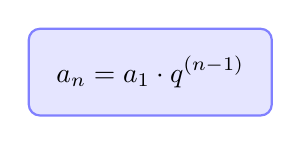
\begin{tikzpicture}
\node[rectangle, fill=blue!10, rounded corners, inner sep=10pt, draw=blue!50, thick] (box) {
$\displaystyle a_n = a_1 \cdot q^{(n-1)}$
};
\end{tikzpicture}

\textbf{Onde:}
\begin{itemize}
\item $a_n$ = termo que queremos
\item $a_1$ = primeiro termo
\item $n$ = posição do termo
\item $q$ = razão (quociente entre termos)
\end{itemize}

\subsection*{Razão da PG}

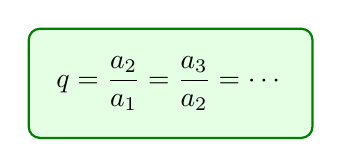
\begin{tikzpicture}
\node[rectangle, fill=green!10, rounded corners, inner sep=10pt, draw=green!50!black, thick] (box) {
$\displaystyle q = \frac{a_2}{a_1} = \frac{a_3}{a_2} = \cdots$
};
\end{tikzpicture}

\subsection*{Soma dos $n$ primeiros termos}

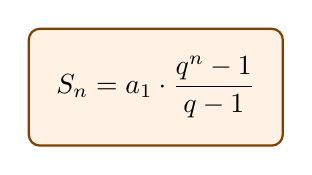
\begin{tikzpicture}
\node[rectangle, fill=orange!10, rounded corners, inner sep=10pt, draw=orange!50!black, thick] (box) {
$\displaystyle S_n = a_1 \cdot \frac{q^n - 1}{q - 1}$
};
\end{tikzpicture}

\section*{Exercícios Básicos}

\begin{enumerate}[leftmargin=*]

\item Determine a razão de cada PG:
\begin{enumerate}[label=\alph*)]
\item $(2, 6, 18, 54, \ldots)$
\item $(81, 27, 9, 3, \ldots)$
\item $(5, -10, 20, -40, \ldots)$
\end{enumerate}

\item Calcule o 5º termo de cada PG:
\begin{enumerate}[label=\alph*)]
\item $(3, 6, 12, 24, \ldots)$
\item $(256, 128, 64, 32, \ldots)$
\item $(1, 4, 16, 64, \ldots)$
\end{enumerate}

\item Encontre o 6º termo das PGs:
\begin{enumerate}[label=\alph*)]
\item $(2, 8, 32, 128, \ldots)$
\item $(1000, 100, 10, 1, \ldots)$
\end{enumerate}

\item Escreva os 4 primeiros termos da PG sabendo que:
\begin{enumerate}[label=\alph*)]
\item $a_1 = 2$ e $q = 3$
\item $a_1 = 64$ e $q = \frac{1}{2}$
\item $a_1 = 5$ e $q = -2$
\end{enumerate}

\item Calcule a soma dos:
\begin{enumerate}[label=\alph*)]
\item 5 primeiros termos da PG $(2, 6, 18, 54, \ldots)$
\item 6 primeiros termos da PG $(3, 12, 48, 192, \ldots)$
\item 4 primeiros termos da PG $(100, 50, 25, 12.5, \ldots)$
\end{enumerate}

\item Interpole 3 meios geométricos entre:
\begin{enumerate}[label=\alph*)]
\item 2 e 32
\item 3 e 48
\end{enumerate}

\item Problemas simples:
\begin{enumerate}[label=\alph*)]
\item Uma PG tem $a_1 = 2$ e $q = 4$. Qual é o 6º termo?
\item Uma PG tem $a_1 = 1000$ e $q = 0,1$. Qual é o 5º termo?
\item Calcule a soma dos 5 primeiros termos da PG $(1, 3, 9, 27, \ldots)$
\end{enumerate}

\item Complete as PGs:
\begin{enumerate}[label=\alph*)]
\item $( \_, 4, 8, 16, \_ )$
\item $(27, \_, 3, \_, \frac{1}{3})$
\item $( \_, 6, 18, 54, \_ )$
\end{enumerate}

\item Determine o número de termos das PGs:
\begin{enumerate}[label=\alph*)]
\item $(2, 6, 18, \ldots, 1458)$
\item $(1024, 512, 256, \ldots, 1)$
\end{enumerate}

\item Problemas do cotidiano:  
\begin{enumerate}[label=\alph*)] 
\item Uma população de bactérias dobra a cada hora. Se inicialmente há 100 bactérias, quantas haverá após 6 horas?
\item Uma bola é lançada de uma altura de 10m. A cada quique, ela sobe 70\% da altura anterior. Qual a altura do 5º quique?
\end{enumerate}

\vspace{10cm}
\hspace{2cm}{\LARGE{\textcolor{blue}{Gabarito}}}
\vspace{10pt}
% Diminui o espaço entre boxes
\tcbset{
  before skip=4pt,
  after skip=4pt,
}
% Questão 1
\begin{tcolorbox}[colback=blue!8,colframe=blue!60!black,title=\textbf{Questão 1 },text width=0.85\columnwidth]
Determine a razão de cada PG: \\
(a) $(2,6,18,54,\ldots)$ \\ (b) $(81,27,9,3,\ldots)$ \\ (c) $(5,-10,20,-40,\ldots)$
\end{tcolorbox}

\begin{tcolorbox}[colback=green!10,colframe=green!60!black,title=\textbf{Solução da questão 1 },text width=0.85\columnwidth]
\textbf{Definição:} $q=\dfrac{a_2}{a_1}$.

(a) $q=\dfrac{6}{2}=3$. Verificação: $\dfrac{18}{6}=3,\ \dfrac{54}{18}=3$. \\
\(\boxed{q=3}\). \\

(b) $q=\dfrac{27}{81}=\dfrac{1}{3}$. Verificação: $\dfrac{9}{27}=\tfrac{1}{3}$. \\
\(\boxed{q=\tfrac{1}{3}}\). \\

(c) $q=\dfrac{-10}{5}=-2$. Verificação: $\dfrac{20}{-10}=-2,\ \dfrac{-40}{20}=-2$. \\
\(\boxed{q=-2}\).
\end{tcolorbox}

% Questão 2
\begin{tcolorbox}[colback=blue!8,colframe=blue!60!black,title=\textbf{Questão 2 },text width=0.85\columnwidth]
Calcule o 5º termo de cada PG: \\
(a) $(3,6,12,24,\ldots)$ \\ (b) $(256,128,64,32,\ldots)$ \\ (c) $(1,4,16,64,\ldots)$
\end{tcolorbox}

\begin{tcolorbox}[colback=green!10,colframe=green!60!black,title=\textbf{Solução da questão 2 },text width=0.85\columnwidth]
Usamos $a_n=a_1\cdot q^{\,n-1}$ com $n=5$.

(a) $q=\dfrac{6}{3}=2$. \\
$a_5 = 3\cdot 2^{4} = 3\cdot16 = \boxed{48}$ \\

(b) $q=\dfrac{128}{256}=\tfrac{1}{2}$. \\
$a_5 = 256\cdot\left(\tfrac{1}{2}\right)^{4} = 256\cdot\tfrac{1}{16} = \boxed{16}$ \\

(c) $q=\dfrac{4}{1}=4$. \\
$a_5 = 1\cdot 4^{4} = \boxed{256}$
\end{tcolorbox}

% Questão 3
\begin{tcolorbox}[colback=blue!8,colframe=blue!60!black,title=\textbf{Questão 3 },text width=0.85\columnwidth]
Encontre o 6º termo das PGs: \\
(a) $(2,8,32,128,\ldots)$ \\ (b) $(1000,100,10,1,\ldots)$
\end{tcolorbox}

\begin{tcolorbox}[colback=green!10,colframe=green!60!black,title=\textbf{Solução da questão 3 },text width=0.9\columnwidth]
(a) $q=\dfrac{8}{2}=4$. \\
$a_6 = 2\cdot 4^{5} = 2\cdot 1024 = \boxed{2048}.$ \\

(b) $q=\dfrac{100}{1000}=0{,}1$. \\
$a_6 = 1000\cdot (0{,}1)^{5} = 1000\cdot 10^{-5} = 1000\cdot 0{,}00001 = \boxed{0{,}01}.$
\end{tcolorbox}

% Questão 4
\begin{tcolorbox}[colback=blue!8,colframe=blue!60!black,title=\textbf{Questão 4 },text width=0.9\columnwidth]
Escreva os 4 primeiros termos da PG sabendo que: \\
(a) $a_1=2,\ q=3$ \\ (b) $a_1=64,\ q=\tfrac{1}{2}$ \\  (c) $a_1=5,\ q=-2$
\end{tcolorbox}

\begin{tcolorbox}[colback=green!10,colframe=green!60!black,title=\textbf{Solução da questão 4 },text width=0.9\columnwidth]
Aplicamos $a_{n}=a_1 q^{n-1}$ para os primeiros termos:

(a) $2,\ 2\cdot3=6,\ 2\cdot3^2=18,\ 2\cdot3^3=54$. \\
\(\boxed{(2,6,18,54)}\).  \\

(b) $64,\ 64\cdot\tfrac12=32,\ 64\cdot(\tfrac12)^2=16,\ 64\cdot(\tfrac12)^3=8$. \\
\(\boxed{(64,32,16,8)}\). \\

(c) $5,\ 5\cdot(-2)=-10,\ 5\cdot(-2)^2=20,\ 5\cdot(-2)^3=-40$. \\
\(\boxed{(5,-10,20,-40)}\).
\end{tcolorbox}

% Questão 5
\begin{tcolorbox}[colback=blue!8,colframe=blue!60!black,title=\textbf{Questão 5 },text width=0.9\columnwidth]
Calcule a soma dos: \\
(a) 5 primeiros termos da PG $(2,6,18,54,\ldots)$ \\
(b) 6 primeiros termos da PG $(3,12,48,192,\ldots)$ \\
(c) 4 primeiros termos da PG $(100,50,25,12.5,\ldots)$
\end{tcolorbox}

\begin{tcolorbox}[colback=green!10,colframe=green!60!black,title=\textbf{Solução da questão 5 },text width=0.9\columnwidth]
Usamos $S_n = a_1\cdot\dfrac{q^{n}-1}{q-1}$ (para $q\neq1$).

(a) $a_1=2$, $q=3$, $n=5$. \\
$S_5 = 2\cdot\dfrac{3^{5}-1}{3-1} = 2\cdot\dfrac{243-1}{2} = 2\cdot\dfrac{242}{2} = \boxed{242}.$

(b) $a_1=3$, $q=4$, $n=6$. \\
$S_6 = 3\cdot\dfrac{4^{6}-1}{4-1} = 3\cdot\dfrac{4096-1}{3} = 3\cdot\dfrac{4095}{3} = \boxed{4095}.$

(c) $a_1=100$, $q=\tfrac{1}{2}$, $n=4$. \\
$S_4 = 100\cdot\dfrac{(\tfrac12)^4 - 1}{\tfrac12 - 1} = 100\cdot\dfrac{\tfrac{1}{16}-1}{- \tfrac12}$. \\
Calcule: $\tfrac{1}{16}-1 = -\tfrac{15}{16}$, dividindo por $-\tfrac12$ dá $(-15/16)/(-1/2)=(-15/16)\cdot(-2)=30/16=15/8$. \\
$S_4 = 100\cdot \tfrac{15}{8} = 125\cdot \tfrac{15}{10} = 187{,}5$ (ou calcule diretamente $100+50+25+12{,}5=187{,}5$). \\
\(\boxed{187{,}5}\).
\end{tcolorbox}

% Questão 6
\begin{tcolorbox}[colback=blue!8,colframe=blue!60!black,title=\textbf{Questão 6 },text width=0.85\columnwidth]
Interpole 3 meios geométricos entre: \\
(a) 2 e 32 \\ (b) 3 e 48
\end{tcolorbox}

\begin{tcolorbox}[colback=green!10,colframe=green!60!black,title=\textbf{Solução da questão 6 },text width=0.85\columnwidth]
Queremos 3 meios → total de 5 termos: $a_1$, $a_2$, $a_3$, $a_4$, $a_5$ com $a_1$ dado e $a_5$ dado. A razão $q=(a_5/a_1)^{1/4}$. \\

(a) $q=(32/2)^{1/4}=(16)^{1/4}=2$. \\
Sequência: $2,\ 4,\ 8,\ 16,\ 32$. \\
Meios geométricos: \(\boxed{4,\ 8,\ 16}\). \\

(b) $q=(48/3)^{1/4}=(16)^{1/4}=2$. \\
Sequência: $3,\ 6,\ 12,\ 24,\ 48$. \\
Meios geométricos: \(\boxed{6,\ 12,\ 24}\).
\end{tcolorbox}

% Questão 7
\begin{tcolorbox}[colback=blue!8,colframe=blue!60!black,title=\textbf{Questão 7 },text width=0.85\columnwidth]
Problemas simples: \\
(a) PG com $a_1=2$, $q=4$. Qual o 6º termo? \\
(b) PG com $a_1=1000$, $q=0{,}1$. Qual o 5º termo? \\
(c) Calcule a soma dos 5 primeiros termos da PG $(1,3,9,27,\ldots)$
\end{tcolorbox}

\begin{tcolorbox}[colback=green!10,colframe=green!60!black,title=\textbf{Solução da questão 7 },text width=0.85\columnwidth]
(a) $a_6 = 2\cdot 4^{5} = 2\cdot 1024 = \boxed{2048}. $ \\

(b) $a_5 = 1000\cdot (0{,}1)^{4} = 1000\cdot 10^{-4} = 0{,} \boxed{0{,}1}.$ \\

(c) $a_1=1$, $q=3$, $n=5$. \\
    $S_5 = 1\cdot\dfrac{3^{5}-1}{3-1} = \dfrac{243-1}{2} = \dfrac{242}{2} = \boxed{121}.$
\end{tcolorbox}

% Questão 8
\begin{tcolorbox}[colback=blue!8,colframe=blue!60!black,title=\textbf{Questão 8 },text width=0.85\columnwidth]
Complete as PGs: \\
(a) $(\_,4,8,16,\_)$ \\ (b) $(27,\_,3,\_,\tfrac{1}{3})$ \\ (c) $(\_,6,18,54,\_)$
\end{tcolorbox}

\begin{tcolorbox}[colback=green!10,colframe=green!60!black,title=\textbf{Solução da questão 8 },text width=0.9\columnwidth]
(a) Observando $4,8,16$ → $q=2$. Então sequência: $2,4,8,16,32$. \\
\(\boxed{(2,4,8,16,32)}\). \\

(b) $27,\_,3,\_,\tfrac{1}{3}$. Aqui $a_1=27$, $a_5=\tfrac{1}{3}$. A razão $q$ satisfaz $27\cdot q^{4}=\tfrac{1}{3}$. \\
$q^{4} = \dfrac{1}{3}\cdot\dfrac{1}{27} = \dfrac{1}{81} \Rightarrow q = \left(\tfrac{1}{81}\right)^{1/4} = \tfrac{1}{3}$. \\
Então termos: $27,\ 9,\ 3,\ 1,\ \tfrac{1}{3}$. \\
\(\boxed{(27,9,3,1,\tfrac{1}{3})}\). \\

(c) $6,18,54$ → $q=3$. Assim sequência: $2,6,18,54,162$ (note que o termo anterior a 6 é $6/3=2$). \\
\(\boxed{(2,6,18,54,162)}\).
\end{tcolorbox}

% Questão 9
\begin{tcolorbox}[colback=blue!8,colframe=blue!60!black,title=\textbf{Questão 9 },text width=0.9\columnwidth]
Determine o número de termos das PGs: \\
(a) $(2,6,18,\ldots,1458)$ \\ (b) $(1024,512,256,\ldots,1)$
\end{tcolorbox}

\begin{tcolorbox}[colback=green!10,colframe=green!60!black,title=\textbf{Solução da questão 9 },text width=0.9\columnwidth]
Usamos $a_n = a_1\cdot q^{\,n-1}$ e resolvemos para $n$.

(a) $a_1=2$, $q=3$ (pois $6/2=3$), queremos $a_n=1458$. \\
$1458 = 2\cdot 3^{\,n-1} \Rightarrow 3^{\,n-1} = \dfrac{1458}{2} = 729 = 3^{6}$. \\
Logo $n-1=6 \Rightarrow n=7$. \\
\(\boxed{7\ \text{termos}}\).

(b) $a_1=1024$, $q=\tfrac{1}{2}$, queremos $a_n=1$. \\
$1 = 1024\cdot \left(\tfrac{1}{2}\right)^{\,n-1} \Rightarrow \left(\tfrac{1}{2}\right)^{\,n-1} = \dfrac{1}{1024} = 2^{-10}$. \\
Assim $n-1=10 \Rightarrow n=11$. \\
\(\boxed{11\ \text{termos}}\).
\end{tcolorbox}

% Questão 10
\begin{tcolorbox}[colback=blue!8,colframe=blue!60!black,title=\textbf{Questão 10 },text width=0.9\columnwidth]
Problemas do cotidiano: \\
(a) Uma população de bactérias dobra a cada hora. Se inicialmente há 100 bactérias, quantas haverá após 6 horas? \\

(b) Uma bola é lançada de uma altura de 10 m. A cada quique, ela sobe 70\% da altura anterior. Qual a altura do 5º quique?
\end{tcolorbox}

\begin{tcolorbox}[colback=green!10,colframe=green!60!black,title=\textbf{Solução da questão 10 },text width=0.85\columnwidth]
Ambos são PGs: (a) $a_1=100$, $q=2$. Após 6 horas → $a_7$? \\

Cuidado: "após 6 horas" significa aplicar a razão 6 vezes; o número é $a_{7}$ se contássemos hora zero como $a_1$. Aqui usamos $a_{6+1}$ quando interpretado assim; por consistência interpretamos: \emph{após 6 horas} = $a_{7}$ se a contagem começa em hora 0, mas se $a_1$ for a quantidade inicial (hora 0), após 6 horas será $a_{7}$. Se $a_1$ for hora 1, após 6 horas será $a_6$. Para evitar ambiguidade, assumimos $a_1$ = quantidade inicial e queremos quantidade após 6 dobramentos $\Rightarrow a_{1}\cdot 2^{6}=100\cdot64 = \boxed{6400}.$ \\

(b) $a_1=10$ m, $q=0{,}7$. Altura do 5º quique = depois de 5 quedas? Interpreta-se como $a_5 = 10\cdot 0{,}7^{5-1}$ se o 1º quique for $a_1$ ou como $10\cdot 0{,}7^{5}$ dependendo da contagem. Aqui tomamos o 1º quique como $a_1=10\cdot0{,}7$ (após primeiro quique), então altura do 5º quique = $10\cdot 0{,}7^{5}$. Calculando: $0{,}7^{2}=0{,}49$, $0{,}7^{3}=0{,}343$, $0{,}7^{4}=0{,}2401$, $0{,}7^{5}=0{,}16807$. \\
Altura $\approx 10\cdot 0{,}16807 = 1{,}6807\ \text{m}$. \\
\(\boxed{\approx 1{,}68\ \text{m}}\).
\end{tcolorbox}

\end{multicols}

\end{document}
